\documentclass{article}
\usepackage{tikz}

\begin{document}

\begin{center}
    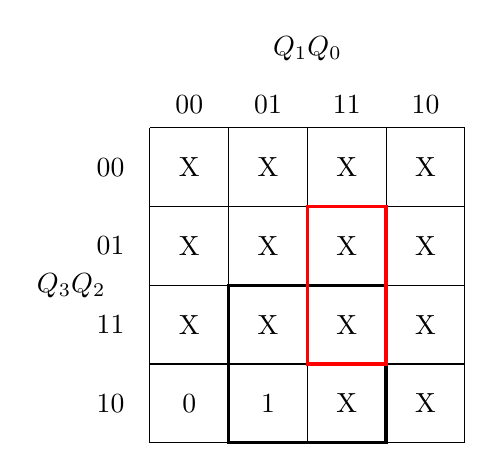
\begin{tikzpicture}
        % Draw the 4x4 Karnaugh map grid
        \draw (0,0) grid (4,4);
        
        % Labels
        \node at (-0.5, 3.5) {$00$};
        \node at (-0.5, 2.5) {$01$};
        \node at (-0.5, 1.5) {$11$};
        \node at (-0.5, 0.5) {$10$};
        
        \node at (0.5, 4.3) {$00$};
        \node at (1.5, 4.3) {$01$};
        \node at (2.5, 4.3) {$11$};
        \node at (3.5, 4.3) {$10$};
        
        % Map values (X placeholders)
        \node at (0.5,3.5) {X}; \node at (1.5,3.5) {X}; \node at (2.5,3.5) {X}; \node at (3.5,3.5) {X};
        \node at (0.5,2.5) {X}; \node at (1.5,2.5) {X}; \node at (2.5,2.5) {X}; \node at (3.5,2.5) {X};
        \node at (0.5,1.5) {X}; \node at (1.5,1.5) {X}; \node at (2.5,1.5) {X}; \node at (3.5,1.5) {X};
        \node at (0.5,0.5) {0}; \node at (1.5,0.5) {1}; \node at (2.5,0.5) {X}; \node at (3.5,0.5) {X};

        % Thick outline for m7, m9, m11, m13, m15
        \draw[black, very thick] (1,0) rectangle (3,2);
        \draw[red, very thick] (2,1) rectangle (3,3);


        % Axis labels
        \node at (-1, 2) {$Q_3 Q_2$};
        \node at (2, 5) {$Q_1 Q_0$};

    \end{tikzpicture}
\end{center}

\end{document}  [K3 Inc]
